
\section{引言}
阵列信号处理技术在许多领域有所运用,维纳滤波是最基础
的阵列信号处理滤波器,其最基本的方法是通过矩阵分解
获得信号处理方程的解。而本文以麦克风阵列信号模型为例通过更加有效的
解方程的CG算法(共轭梯度法)直接获得其维纳解。在保证其准确性的情况下算法耗时有大幅度减少。
本文由以下部分构成:第2节介绍信号模型和维纳滤波技术。第3节介绍经典
维纳滤波矩阵求解方式。第4节介绍本文所要复现的共轭梯度的方法求解
维纳滤波矩阵。第5章给出仿真实验结果,最后给出一些结论。第6章为本次大作业
的心得体会。

我们小组分工明确,认真完成了复现工作,具体的分工如下::
\begin{itemize}
\item
查阅讨论文献(一起)
\item{代码部分}:
 邱梁城
\item{传统方法复现}:邱梁城,严铮
\item{报告} \\
\textbf{严铮}:
摘要,引言(1),信号模型 (2)和经典求解维纳滤波器(3.1),算法仿真(5)和参考文献\\
\textbf{邱梁城}:
衡量指标(3.2),基于共轭梯度法的快速算法(4),仿真结果(5),参考文献和最终整理\\ 
\end{itemize}

\section{信号模型与维纳滤波}
\subsection{信号模型}
一个具有N个通道的麦克风阵列系统,第n个通道在t时刻接收到的含噪声语言信号模型
\begin{align}
	y_n(t) &= \mathbf{g_n} \ast \mathbf{s}(n) + \mathbf{v_n}(t) \\
	&= \mathbf{x_n}(t) + \mathbf{v_n}(t); \quad n=1,2,\ldots,N
\end{align}

其中$g_n$表示从信号源到第n个麦克风系统传输函数,*表示卷积,$x_n(t)$和$v_n(t)$分别表示麦克风接收到的信号成分及加性噪声,且通常假设噪声与语言不相关。

语言增强的目的是由这N个通道收到的带噪语音信号,提取出目标的语音信号,一般把$x_1(t)$作为目标信号。多通道语言增强算法\cite{ref1}主要基于线性滤波器,即计算线性滤波器矩阵$H$使得通过滤波器后的信号估计为$z=HY$其中Y为收到的含噪声语言信号。
将其用向量形式表示如下
\begin{align}
		y_{n}(k)&=x_{n}(k)+v_{n}(k), \quad n=1,2, \ldots . N \\
		y_{n}(k)&=\left[\mathrm{y}_{\mathrm{n}}(\mathrm{k}) \mathrm{y}_{\mathrm{n}}(\mathrm{k}-1) \ldots \mathrm{y}_{\mathrm{n}}(\mathrm{k}-\mathrm{L}+1)\right]^{T} \\
		x_{n}(k)&=\left[\mathrm{x}_{\mathrm{n}}(\mathrm{k}) \mathrm{x}_{\mathrm{n}}(\mathrm{k}-1) \ldots \mathrm{x}_{\mathrm{n}}(\mathrm{k}-\mathrm{L}+1)\right]^{T} \\
		v_{n}(k)&=\left[\mathrm{v}_{\mathrm{n}}(\mathrm{k}) \mathrm{v}_{\mathrm{n}}(\mathrm{k}-1) \ldots \mathrm{v}_{\mathrm{n}}(\mathrm{k}-\mathrm{L}+1)\right]^{T}
\end{align}

\begin{figure}[h]
	\centering
	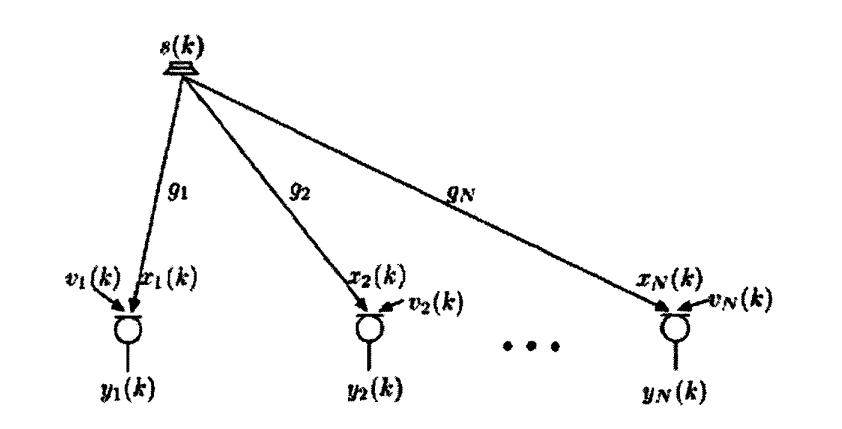
\includegraphics[width=0.5\textwidth]{mod.PNG}
	\caption{信号模型}
	\label{mod}
\end{figure}
$x_n(k)$和$v_n(k)$分别表示麦克风接收到的语言信号和加性噪声,L为滤波阶数,令$H$为线性滤波器
则第一道语言估计为
\begin{equation}
	z(k)=\mathbf{HY(k)}
\end{equation}
\begin{equation}
	z(k)=\mathbf{HY(k)}=\mathbf{H[X(k)+V(k)]} \label{3}
\end{equation}
其中:
\begin{equation}
	Y(k)=[y_1^T\  y_2^T\ldots y_n^T]^T
\end{equation}
\begin{equation}
	X(k)=[x_1^T x_2^T\ldots x_n^T]^T
\end{equation}
\begin{equation}
	V(k)=[v_1^T \ v_2^T\ldots\  v_n^T]^T
\end{equation}
\begin{equation}
	H=[h_1^T\ h_2^T\ldots\ h_n^T]
\end{equation}
$h_n(n=1,2\ldots N)$为L*L阶滤波矩阵,我们定义估计的信号误差为:
\begin{align}
	e(k) &= z(k) - x_1(k) \\
	&= (H-Q)X(k) + HV(k) \\
	&= e_x(k) + e_v(k)
\end{align}
其中\[ Q=[I_{L*L}\ 0_{L*L}\ldots\ 0_{L*L}] \]
是一个$N*NL$且$I_{L*L}$是为$L*L$的单位矩阵
\subsection{维纳滤波器}
	根据上节信号模型,则估计的信号最小二乘误差(MSE)的表达式
\begin{align}
	J(W) &=tr{E[e(k)e(k)^T]}\\ &=E[x_1(k)x_1(k)^T]+tr[HR_{yy}H^T]-2tr[HR_{yx_1}]
\end{align}
其中
\begin{equation}
	R_{yy}=E[Y(k)Y^T(k)]
\end{equation}
\begin{equation}
	R_{yx_1}=E[Y(k){x_1}^T(k)]
\end{equation} 
将上式$J(H)$对H求偏导,使估计信号误差最小
\begin{equation}
	\frac{\partial J(H)}{\partial H}=0
\end{equation}
得到维纳滤波矩阵
\begin{equation}
	H^T_{wiener}=R^{-1}_{yy}R_{yx_1}
\end{equation}
由于$x_1(k)$无法观测但可知$R_{yx_1} =R_{yy}-R_{vv}$ \cite{ref5}
其中
\begin{equation}
	R_{vv}=E[V(k)V^T(k)] \label{4}
\end{equation}
由此$R_{yy}$和$R_{vv}$为噪声自相矩阵都可以得到
将其带入公式即可求得维纳滤波矩阵。
\section{经典求解维纳滤波矩阵}
这一节中我们将介绍所复现的论文中所运用的求解维纳滤波矩阵算法,同时给出评价滤波器性能的指标,包括ISNR,OSNR,在陈景东教授的书中有很好的介绍。
\subsection{求解维纳滤波矩阵} 
由于$R_{vv}$是一个满秩矩阵,对称矩阵$R_vv$与$R_xx$可联合对角化
\begin{equation}
	T^TR_{xx}T=\Lambda \label{5}
\end{equation}
\begin{equation}
	T^TR_{vv}T=I_{NL} \label{6}
\end{equation}
$\wedge=diag[\lambda_1 \ \lambda_2\ldots\ \lambda_	{NL}]$
由矩阵$R_{vv}^{-1}R_{xx} $的特征值组成且$\lambda_1\ge \lambda_2\ge \ldots \lambda_{NL} \ge 0$,$T$为特征向量$t_1\ t_2\ldots \ t_{NL}$对应组成的矩阵其是一个满秩矩阵,则
\begin{equation}
	t_i^Tx(t)=0,i=n+1\ n+2\ldots NL
\end{equation}
\begin{equation}
	R_{vv}{-1}=\sum\limits_{i=1}^{NL}{{t_it_i^T}}
\end{equation}
\begin{equation}
	R_{vv}^{-1}R_{xx}T=T\Lambda
\end{equation}
\begin{equation}
	T^TR_{yy}T=I_{NL}+\Lambda \label{7}
\end{equation}
我们能够将滤波矩阵$H$化为$H=AT^T$\\
根据上一节定义估计值与真实值误差为$e(k)=z(k)-x_1(k)=AT^Ty(t)-x_1(t)$,我们推断MSE准则变为:
\begin{equation}
	J(A)=tr[R_{x_1}-2AT^TR_{xx}I^T_i+A\Lambda A^T] 
\end{equation}
对$A$求偏导使MSE最小化得到$A_w=I_iT^{-T}\Lambda(\Lambda+I_{NL})^{-1}$
而 $A_WT^T=H_W$其中$H_W$即为维纳滤波矩阵,至于T的求解,我们可以联合利用Cholesky\cite{ref9} 分解与Schur\cite{ref10}分解,求得方程组中的$T$与$\Lambda$,进而求取滤波矩阵$H_W$
最终得到
\begin{equation}
	H_W=I_iR_{xx}\sum\limits_{i=1}^{NL}{\frac{t_it_i^T}{1+\lambda_i}}=
	I_iR_{vv}\sum\limits_{i=1}^{NL}{\frac{\lambda_i}{1+\lambda_i}t_it_i^T}
\end{equation}
\subsection{衡量指标}
在本小节中,我们定义了一些基本度量 \cite{ref13},这些度量很好地描述阵列传感器和线性滤波矩阵的优劣。我们假设传感器1是参考传感器,那么我们定义:\\
输入的SNR(信噪比)为:
\begin{equation}
iSNR=\frac{tr(R_{x1})}{tr(R_{v1})} 
\end{equation}
其中$\mathbf{R}_{\mathbf{x}_{1}}=E\left[\mathbf{x}_{1}(t) \mathbf{x}_{1}^{T}(t)\right]$  和  $\mathbf{R}_{\mathbf{v}_{1}}=E\left[\mathbf{v}_{1}(t) \mathbf{v}_{1}^{T}(t)\right] $ 是$x_1(t)$ 和$y_1(t)$ 的自相关矩阵, 我们知道由于$x_1(t)$不能直接通过传感器获得,我们将直接获得输入信噪比依据 $\mathbf{y}_{1}(t)$ , 其中  $\mathbf{R}_{\mathbf{y}_{1}}=   \mathbf{R}_{\mathbf{x}_{1}}+\mathbf{R}_{\mathbf{v}_{1}} $ \\
我们根据公式\ref{3}能够得知:
\begin{equation}
\begin{align}
R_z&=E[z(t)z^T(t)] \\
&=HR_{yy}H^T \\
&=HR_{xx}H^T+HR_{vv}H^T \\
&=R_{xfd}+R_{vrd}
\end{align}
\end{equation}
此时输出信噪比便可以很容易的获得:
\begin{equation}
	\begin{align}
		oSNR(H)&=\frac{tr(R_{xfd})}{tr(R_{vfn})} \\
		&=\frac{tr(HR_{xx}H^T)}{tr(HR_{vv}H^T)}
	\end{align}
\end{equation}
信噪比增益为:
\begin{equation}
		G_W=\frac{oSNR}{iSNR} 
\end{equation}
到此已经可以很好的描述滤波矩阵以及线性阵列的优劣问题,但是我们希望能够获得维纳滤波矩阵对于噪声以及信号单独的作用效果,我们定义降噪系数如下:
\begin{equation}
\xi _n(H)=\frac{tr(R_{v1})}{tr(R_{vrd})}  
\end{equation}
由于期望的信号可能被滤波矩阵失真,我们定义所需信号衰减因子为:
\begin{equation}
	\xi _n(H)=\frac{tr(R_{x1})}{tr(R_{xfd})}  
\end{equation}

\section{基于共轭梯度法的快速算法}
求解大型线性矩阵已经成为了当前工业所要解决的巨大问题,其中已经有很多成熟的算法,包括由kryov子空间引出的一系列算法,速度快、精度高使得他们被多次运用在大型矩阵的运算,其中共轭梯度法\cite{ref8}具有内存小、收敛速度极快,可通过误差大小控制解的精确度,这一节中,我们将探讨其在维纳滤波矩阵求解过程中的运用。
\subsection{维纳滤波线性方程分析}
对于求解滤波器方程组:$H=R_{yy}^{-1}R_{yx_1}$,考虑到我们无法直接观测到$X1$,所以我们需要对上式进行处理。我们可以很容易地根据公式\ref{4}得出:
\begin{equation}
	R_{yx_1}=(R_{yy}-R_{vv})Q^T
\end{equation}
其中$R_{vv}$为$NL*NL$的矩阵,它可以在静音段利用VDA技术\cite{ref5}估计得到。于是$H$的求解只取决于$R_{yy}$和$R_{vv}$,可以表示为:
\begin{equation}
	H=Q\left(I_{N L}-R_{y y}{ }^{-1} R_{v v}\right)^{T}
\end{equation}
我们考虑使用CG算法进行优化。根据公式\ref{5}、\ref{6}、\ref{7}我们可以很清楚地知道$R_{yy}$是一个对称正定矩阵(特征值均大于0)。
我们构建如下方程组:
\begin{equation}
	R_{yy}H=(R_{yy}-R_{vv})Q^T
\end{equation}
其中$H$是一个NL*L的矩阵,设$M=(R_{yy}-R_{vv})Q^T$,是一个NL*L的矩阵。那么,此方程组便可以按照如下方式求解:
\begin{equation}
	R_{yy}*[h_1 \ h_2 \ h_3 \dots h_L]=[m_1 \ m_2 \ m_3 \dots m_L]
\end{equation}
\subsection{CG算法求解}
接下来我们将要对式进行求解,考虑到CG算法是对线性方程组求解的算法我们将分别对$R_{yy}*h_i=m_i$进行求解。构建一组彼此关于$R_{yy}$共轭的正交基$P1, P2, P3, \dots, P_{n}$,则目标向量可以表示成这组基的线性组合:
\begin{equation}
	H_i=\sum_{j=1}^{n}a_jP_j
\end{equation}
即:
\begin{equation}
	R_{yy}*h_i=m_i=\sum_{j=1}^{n}a_jR_{yy}P_j 
\end{equation}
\begin{equation}
	P_{k}^{T}m_i=a_kP_k^{T}R_{yy}P_{k}
\end{equation}
其中:
\begin{equation}
	a_{k}&=\frac{(P_k,m_i)}{(P_k,P_k){R{yy}}}       &=\frac{P_k^Tm_i}{P_k^TR_{yy}P_k}
\end{equation}
问题变为求解$P$,便可以求出$a_k$和$h_i$。\\
我们假设有一组线性无关的向量组 $y_0, y_1, \dots, y_k$,尝试构造一组$A$共轭的向量组 $P_0, P_1, \dots, P_k$,使其满足:
\begin{equation}
	\operatorname{span}\{y_{0}, y_{1}, \ldots, y_{k}\}=\operatorname{span}\{P_{0}, P_{1}, \ldots, P_{k}\}
\end{equation}
我们这里应用施密特正交化思想,使用迭代法实现$P$的选取。算法步骤如下:
其中$(x_k)$代表第$k$步的迭代向量

步骤一:给定初值$x_0=0$,计算出初始残差:
\begin{equation}
	r_0=m_i-R_{yy}x_0
\end{equation}

步骤二:取$P_0=r_0$,计算得到$x_1$
\begin{equation}
	x_1=x_0+a_0P_0, \quad a_0=\frac{(r_0,P_0)}{(R_{yy}P_0,P_{0})}
\end{equation}

步骤三:由$x_1$得到新的残差$r_1=m_i-R_{yy}x_1$,并以$r_1$为基础,对$P_0$做$A$的投影得到新的前进方向$P_1$
\begin{equation}
	P_1=r_1-\beta_1 P_0,\quad 
\end{equation}
\begin{equation}
\beta_1=\frac{(R_{yy}P_0,r_1)}{(R_{yy}P_0,P_0)}= \frac{r_{k+1}^T r_{k+1}}{r_k^T r_k} 
\end{equation}

步骤四:重复步骤三得到新的迭代向量与残差
\begin{equation}
	\begin{aligned}
		x_{k+1} = x_k+a_kP_k, a_k&=\frac{(r_k,P_k)}{(R_{yy}P_k,P_k)}= \frac{r_k^T r_k}{p_k^T R_{yy} P_k} \\
		r_{k+1} &\to P_{k+1} \to x_{k+2}
	\end{aligned}
\end{equation}

算法伪代码如下:
\begin{algorithm}[H]
	\caption{共轭梯度法}
	\begin{algorithmic}[1] %每行显示行号
		\Require $R_{yy}$:一个 $NL \times NL$ 的对称正定矩阵;$m_i$:一个 $NL \times 1$ 的向量;$x_0$:一个 $NL \times 1$ 的向量,用于初始化
		\Ensure $x$:一个 $NL \times 1$ 的向量,表示方程 $R_{yy}h_i = m_i$ 的解\\
		\textbf{初始化:}\
		\State $r_0 =m_i - R_{yy}x_0$
		\State $p_0 = r_0$
		\State $k = 0$
		\While{未收敛}
		\State $\alpha_k = \frac{r_k^T r_k}{p_k^T R_{yy} p_k}$
		\State $x_{k+1} = x_k + \alpha_k p_k$
		\State $r_{k+1} = r_k - \alpha_k R_{yy} p_k$
		\State $\beta_k = \frac{r_{k+1}^T r_{k+1}}{r_k^T r_k}$
		\State $p_{k+1} = r_{k+1} + \beta_k p_k$
		\State $k = k + 1$
		\EndWhile
		\State \textbf{输出} $x$
	\end{algorithmic}
\end{algorithm}
由此得到的满足误差条件的$x_k$便为我们所需的$h_i$,能够证明由此算法产生的向量序列$r_l$,$P_l$满足:
\begin{equation}{l}
	r_{l} \perp \operatorname{span}\left\{r_{0}, r_{1}, \cdots r_{l-1}\right\} 
\end{equation}
\begin{equation}
	P_{l} \perp \operatorname{span}\left\{P_{0}, P_{1}, \cdots P_{l-1}\right\} 
\end{equation}
\begin{equation}
	\begin{aligned}
	&\operatorname{span}\left\{r_{0}, r_{1}, \cdots r_{l-1}\right\}\\
=&\operatorname{span}\left\{P_{0}, P_{1}, \cdots P_{l-1}\right\}\\
	=&\operatorname{span}\left\{r_{0}, A r_{0}, \ldots, A^{l-1} r_{0}\right\}
	\end{aligned}
\end{equation}
其中 $\operatorname{span}\left\{r_{0}, A r_{0}, \ldots, A^{l-1} r_{0}\right\}$ 为krylov子空间\cite{ref14}
我们对每一个$h_i$进行迭代求解,最终可以得到滤波器$H$的输出。
\section{算法仿真对比}
书中4.21给出了一个例子,本文从该例子着手进行算法的仿真与对比
假定一个随机信号$x(t)=A\cos(2\pi f_0t+\phi )$其中A与$f_0$给定
$ \phi \sim U(0,2\pi )$
假定干扰信号$u(t)$为高斯白噪声即$u(t) \sim \mathcal N(0,{\sigma^2 u})$且信号与$x(t)$不相关,
传感器包含热高斯噪声$w_m(t) \sim \mathcal N(0,\sigma^2 w))$。收到的信号为	$y_m(t)=x_m(t)+v_m(t),m=1,2\ldots M $,其中 $v_m(t)=w_m(t)+u_m(t),m=1,2\ldots M $
$v_m(t)$为加性噪声。 
\begin{equation}
	[R_{x_1}]_{i,j}=\frac{1}{2}A^2\cos[2\pi f_0(i-j)]
\end{equation}
\begin{equation}
	iSNR=10\log\frac{A^2}{\sigma^2 u+\sigma^2 w}(dB)
\end{equation}
给出条件$A=0.5,f_0=0.1,\sigma^2 u=0.5,\sigma^2 w=0.01\sigma^2 u$则iSNR=6.06dB
选择上文提到的$G(H)$与$J(H)/L$作为衡量指标,以CG算法求解维纳滤波矩阵进行仿真实验。并通过改变滤波阶数与传感器个数验证两者对于还原信号的影响。结果如图\ref{333}、\ref{444}所示:
\begin{figure}[ht]
	\centering
	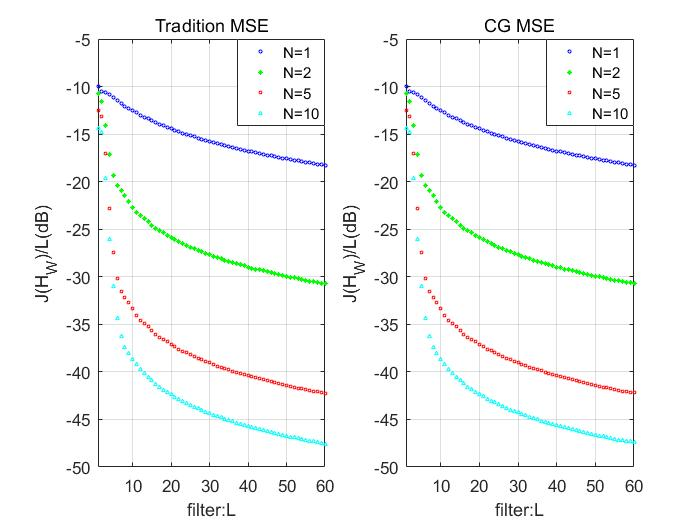
\includegraphics[width=\linewidth,height=5.82cm]{pic/gain.jpg}
	\caption{不同算法下维纳滤波后的误差}
	\label{333}
\end{figure}
\begin{figure}[ht]
	\centering
	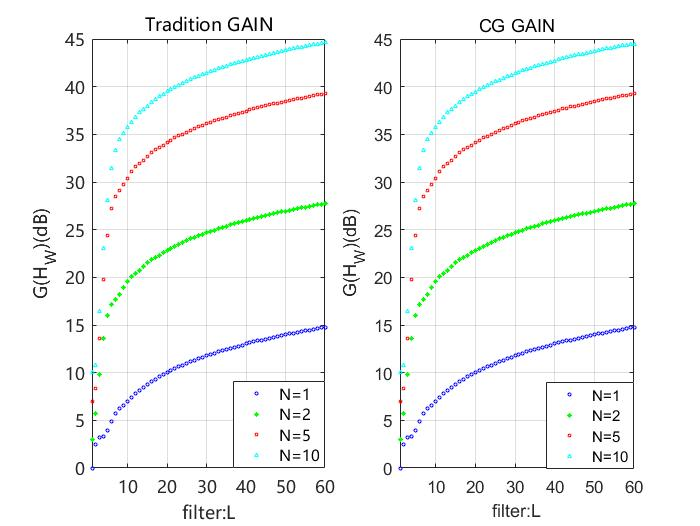
\includegraphics[width=\linewidth,height=5.82cm]{pic/mse.jpg}
	\caption{不同算法下 维纳滤波矩阵对于信号的增益}
	\label{444}
\end{figure}

能够发现CG算法的运用并不会降低滤波器求解矩阵的精确度,其效果与传统算法相当,并且能够从结果图中看到随着滤波阶数与传感器个数的增多,我们对于信号的$G_w$能够有效的提高,并且滤波后的信号与期望信号的误差会随着两者的增加逐渐减小,反映了多阵列传感器能够对语音信号有更好的增强。

接着我们在保证滤波阶数不变的时候改变传感器个数,以此获得两种算法在不同传感器个数下的运行时间:
\begin{table}[hbt]
	\caption{算法运行时间}
	\centering
	\begin{tabular}{ccccc}
		\toprule
		 & N=1 & N =5& N=10& N=50\\
		\midrule
		CG& 0.0036& 0.0029 & 0.0063& 2.9311\\
		tradition&0.0053&0.0059&0.1272& 10.3927\\
		\bottomrule
	\end{tabular}
	\label{tab:label}
\end{table}

我们能够发现CG算法能够明显的改善求解维纳滤波矩阵的运算复杂度,同时也能够保持较高的精度,为了进一步验证维纳滤波器分别对于信号与噪声的作用,我们改变输入信噪比的大小,并且保证滤波阶数L为30,求得传感器个数对于降噪系数与信号衰减因子的影响。
\begin{figure}[ht]
	\centering
	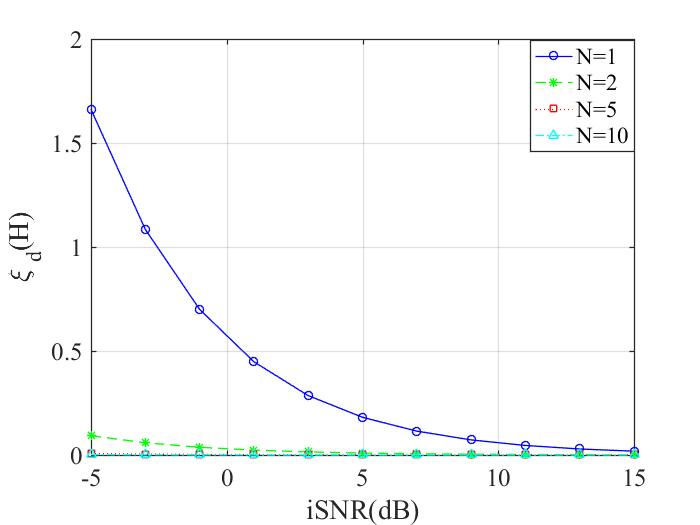
\includegraphics[width=\linewidth,height=5.82cm]{pic/111.jpg}
	\caption{传感器个数对于信号衰减因子的影响}
	\label{111}
\end{figure}
\begin{figure}[ht]
	\centering
	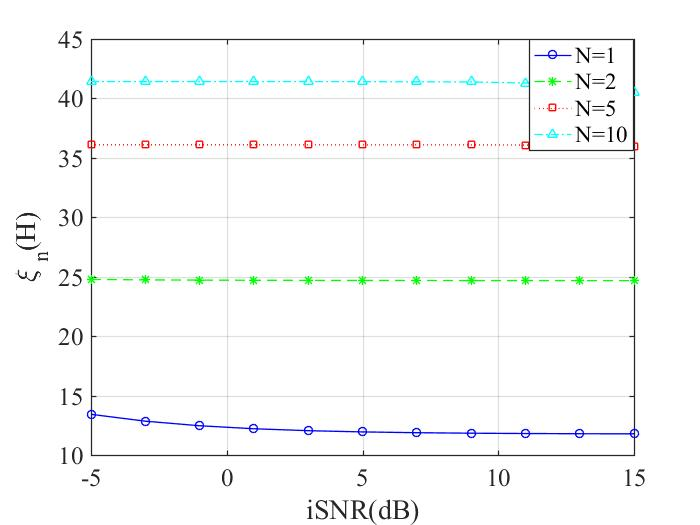
\includegraphics[width=\linewidth,height=5.82cm]{pic/222jpg.jpg}
	\caption{传感器个数对降噪系数的影响}
	\label{222}
\end{figure}

结果如图\ref{111},图\ref{222}所示,能够发现随着传感器个数的增多,维纳滤波器对噪声的抑制效果会逐渐变好,并且对于信号的恢复也有更令人满意的效果。


\section{心得体会}
\subsection{心得体会一/邱梁城}
写到这里计算方法这门课也告一段落了。

回顾起这学期课堂,从一开始接触计算方法的兴奋,到遇见晦涩难懂公式时的沉闷,再到能够实际应用这些方法时的宽慰,庆幸自己坚持了下来。

张老师的这门课让我学习到了很多概念和算法知识,各类的插值法、海森伯格矩阵、CG算法、krylov space等等,之前自己对深度学习有着很大兴趣,但是却没有深入的了解里面的算法原理、如何实现这门课的学习让我能对原理开始进行剖析,再懵懂的工程实践中让我能够有一把自己的匕首攻克难题。再深度算法的学习过程中,共轭梯度算法是一个很重要的内容,但是之前一直一知半解,借着这次大作业的机会,通过查找文献,动手实践,终于能够将其解决。

对于我来说,这门课最大的收获并不在于算法知识的进展和积累,张老师再课堂上不断提起的创新意识、思考意识才是让我受益终身的思想,通过课堂上的问题深入,让我们能够有着自己思考的机会和过程,十分难得宝贵。

数学是思考者的天堂,这句话现在越发感觉正确,对于以前来说,没有考虑过在工程中该如何解决大型线性方程组的求解问题,似乎只会暴力求解,但是无论是这学期所学的LU分解、特征值求解、choloesy分解等等均是快速高效的算法,但是时常质问自己,换做我又是否能想出这些算法或是在这些算法上更近一步,能思考、会思考才是他们与我们的不同,这门课在学习思想上的教育远远大于这门课本身。


此外,在最后的大作业中,调研,仿真,撰写报告的流程,其实和我们做研究的过程很像,在一次次的报错中进步,学习才是科研本身的魅力所在。

由衷的感谢张老师在这一学期中对我的教诲!
\subsection{心得体会二/严铮}
我觉得这节课最重要的就是让我明白可以用迭代的方法求出工程问题的数值解,为解决问题提供了一些新思路。对于本次大作业,一开始有些许害怕,因为大作业有许多部分组成,但通过查阅资料,交流与讨论,最终豁然开朗。对于之前只用过word文档的我来说,latex的使用还是很令人头疼,好在通过学习网上学习资料,也算是成为了入门新手。总之我觉得本次课程让我受益匪浅,而在完成作业的同时也学习到了很多别的东西,相信一定会对以后的学习有所帮助。


